%------------------------------------------------------------------------------
% CV in Latex
% Author : Anindya Kanti Mitra
% Based off of: https://github.com/sb2nov/resume and Jake's Resume on Overleaf 
% License : MIT
%------------------------------------------------------------------------------

\documentclass[11pt]{article}
%\documentclass[letterpaper,11pt]{article} %For use in US
\usepackage{latexsym}
\usepackage[empty]{fullpage}
\usepackage{titlesec}
\usepackage{marvosym}
\usepackage[usenames,dvipsnames]{color}
\usepackage{verbatim}
\usepackage{enumitem}
\usepackage[hidelinks]{hyperref}
\usepackage[english]{babel}
\usepackage{tabularx}
\usepackage{tikz}
\usepackage{lastpage}
\usepackage{fancyhdr}
\pagestyle{fancy}
\input{glyphtounicode}


%-----FONT OPTIONS-------------------------------------------------------------

% serif
 \usepackage{palatino}
% \usepackage{times} %This is the default as well
% \usepackage{charter}

% sans-serif
% \usepackage{helvet}
% \usepackage[sfdefault]{noto-sans}
% \usepackage[default]{sourcesanspro}

%-----PAGE SETUP---------------------------------------------------------------

% Adjust margins
\addtolength{\oddsidemargin}{-1cm}
\addtolength{\evensidemargin}{-1cm}
\addtolength{\textwidth}{2cm}
\addtolength{\topmargin}{-1.5cm}
\addtolength{\textheight}{3cm}

% Margins for US Letter size
%\addtolength{\oddsidemargin}{-0.5in}
%\addtolength{\evensidemargin}{-0.5in}
%\addtolength{\textwidth}{1in}
%\addtolength{\topmargin}{-.5in}
%\addtolength{\textheight}{1.0in}

\urlstyle{same}

\raggedbottom
\raggedright
\setlength{\tabcolsep}{0cm}

% Sections formatting
\titleformat{\section}{
  \vspace{-4pt}\scshape\raggedright\large
}{}{0em}{}[\color{black}\titlerule \vspace{-5pt}]

% Ensure that .pdf is machine readable/ATS parsable
\pdfgentounicode=1

%-----CUSTOM COMMANDS FOR FORMATTING SECTIONS----------------------------------
\renewcommand{\headrulewidth}{0pt}
\fancyhead{}
\fancyfoot[C]{ Page - \thepage\ of \pageref{LastPage}}
 \setlength{\footskip}{14pt}
\newcommand{\CVItem}[1]{
  \item\small{
    {#1 \vspace{-2pt}}
  }
}

\newcommand{\CVSubheading}[4]{
  \vspace{-2pt}\item
    \begin{tabular*}{0.97\textwidth}[t]{l@{\extracolsep{\fill}}r}
      \textbf{#1} & #2 \\
      \small#3 & \small #4 \\
    \end{tabular*}\vspace{-7pt}
}

\newcommand{\CVSubSubheading}[2]{
    \item
    \begin{tabular*}{0.97\textwidth}{l@{\extracolsep{\fill}}r}
      \text{\small#1} & \text{\small #2} \\
    \end{tabular*}\vspace{-7pt}
}

\newcommand{\CVSubItem}[1]{\CVItem{#1}\vspace{-4pt}}

\renewcommand\labelitemii{$\vcenter{\hbox{\tiny$\bullet$}}$}

\newcommand{\CVSubHeadingListStart}{\begin{itemize}[leftmargin=0.5cm, label={}]}
% \newcommand{\resumeSubHeadingListStart}{\begin{itemize}[leftmargin=0.15in, label={}]} % Uncomment for US
\newcommand{\CVSubHeadingListEnd}{\end{itemize}}
\newcommand{\CVItemListStart}{\begin{itemize}}
\newcommand{\CVItemListEnd}{\end{itemize}\vspace{-5pt}}

%------------------------------------------------------------------------------
% CV STARTS HERE  %
%------------------------------------------------------------------------------
\begin{document}

%-----HEADING------------------------------------------------------------------
\begin{comment}
Display Picture included here
\end{comment}

\begin{minipage}[c]{0.05\textwidth}
\-\
\end{minipage}
\begin{minipage}[c]{0.2\textwidth}
\begin{tikzpicture}
    \clip (0,0) circle (1.2cm);
    \node at (0,-.5) {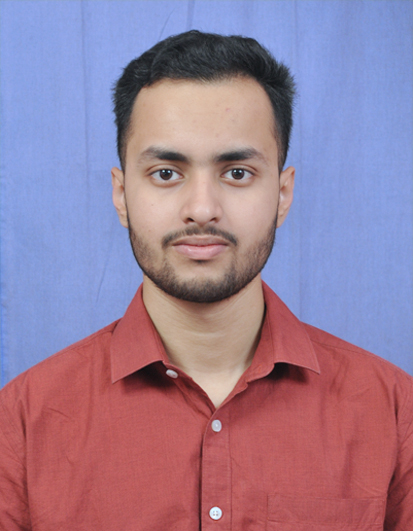
\includegraphics[width = 2.65cm]{photo.jpg}}; 
    % if necessary the picture may be moved by changing the at (coordinates)
    % width defines the 'zoom' of the picture
\end{tikzpicture}
%\hfill\vline\hfill
\end{minipage}
\begin{minipage}[c]{0.6\textwidth}
    \textbf{\Huge \scshape{Anindya Kanti Mitra}} \\ \vspace{1pt} 
    % \scshape sets small capital letters, remove if desired
    %\small{phone number} \\
    \href{mailto:anindya15d12m@gmail.com}{anindya15d12m@gmail.com}\\
    % Be sure to use a professional *personal* email address
    \href{https://www.linkedin.com/in/anindyamitra15/}{linkedin.com/in/anindyamitra15} \\
    % you should adjust you linked in profile name to be professional and recognizable
    \href{Tel:+919330665498}{+91 933-066-5498}
\end{minipage}

\begin{comment}
I am passionate about electronics and have expertise in it. I have worked on personal projects on power, analog, and digital electronics. I’ve also worked with microcontrollers for companies, which I’ve mentioned in this CV. As a plus, I also know how to work with Linux environments and programming in several languages.
\end{comment}

%-----EDUCATION----------------------------------------------------------------
\section{Education}
  \CVSubHeadingListStart
%    \CVSubheading % Example
%      {Degree Achieved}{Years of Study}
%      {Institution of Study}{Where it is located}
    \CVSubheading
      {{Master of Technology $|$ \emph{\small{VLSI Design}}}}{Aug. 2023 -- July 2025}
      {Indian Institute of Engineering Science \& Technology}{Shibpur, Howrah}
    \CVSubheading
      {{Bachelor of Technology $|$ \emph{\small{Electronics \& Communication Engineering}}}}{Aug. 2019 -- July 2023}
      {Kalyani Govt. Engineering College}{Kalyani, Nadia}
  \CVSubHeadingListEnd

%-----WORK EXPERIENCE----------------------------------------------------------
\section{Work Experience}
  \CVSubHeadingListStart
%    \CVSubheading %Example
%      {What you did}{When you worked there}
%      {Who you worked for}{Where they are located}
%      \CVItemListStart
%        \CVItem{Why it is important to this employer}
%      \CVItemListEnd
	\CVSubheading
      	{GenC Next Programmer Analyst Trainee}{February 2023 -- July 2023}
      	{Cognizant Technology Solutions}{Candor Tech Space, Newtown, Kolkata}
      \CVItemListStart
       \CVItem{Worked with React-js, Springboot microservice based architecture}
    \CVItemListEnd
    \CVSubheading
      {IoT Engineer}{July 2022 -- January 2023}
      {Mind Webs Ventures}{Sector-V, Salt Lake, Kolkata}
      \CVItemListStart
        \CVItem{Made and maintained projects on Node-js backend and Angular frontend}
        \CVItem{Made IoT projects involving ESP32, ESP8266, RFID sensors and WiFi HTTP and SocketIO}
    \CVItemListEnd
    \CVSubheading
      {PCB Designer Intern}{June 2021 -- November 2021}
      {Adben Industries Pvt. Ltd.}{Kolkata}
      \CVItemListStart
        \CVItem{Designed multi-layer PCB for an IoT device on KiCAD}
        \CVItem{Designed 4-layered SMD PCB for a smart-watch}
      \CVItemListEnd

    
  \CVSubHeadingListEnd


%-----SKILLS-------------------------------------------------------------------
\section{Skills}
 \begin{itemize}[leftmargin=0.5cm, label={}]
    \small{\item{
     \textbf{Languages}{: English, Bengali (Native), Hindi} \\
     \textbf{Programming}{: Python, MATLAB, Java, C/C++, Arduino, Verilog, HTML, JS, Tcl} \\
     \textbf{Document Creation}{: Microsoft Office Suite, LaTex, Markdown} \\
     \textbf{Tools}{: Xilinx ISE / Vivado, Cadence Virtuoso, KiCAD, EasyEDA, LTSpice, ESP-IDF, PlatformIO, Node-js, Firebase, STMCube IDE, Eclipse, VS Code, Git} \\
    }}
 \end{itemize}

%-----PROJECTS AND RESEARCH----------------------------------------------------
\section{Projects and Research}
  \CVSubHeadingListStart
%    \CVSubheading
%      {Title of Work}{When it was done}
%      {Institution you worked with}{unused}

    \CVSubheading
      {{Opamp and Comparator design on SCL 180nm PDK} $|$ \emph{\small{Cadence Virtuoso Spectre}}}{Summer 2024}
      {IIEST Shibpur}{}
    \CVItemListStart
      \CVItem{Two stage and folded cascode opamp design}
      \CVItem{Dynamic Comparator with calibration}
    \CVItemListEnd 
    
    \CVSubheading
      {{IoT Water Management System and Home Automation} $|$ \emph{\small{B.Tech Final Project}}}{Summer 2023}
      {Kalyani Govt. Engineering College}{}
    \CVItemListStart
        \CVItem{ESP32, Socket IO (WebSocket), WiFi, Node-js based full stack IoT home automation project from scratch}
        \CVItem{Programmable capacitive water level sensing and programmable intelligent IoT water pump and schedule based appliance control}
    \CVItemListEnd      
      
    \CVSubheading
      {{WiFi based autonomous bot control system with computer vision} $|$ \emph{\small{Python, Cpp}}}{Autumn 2021}
      {Flipkart GRiD 3.0 Robotics Challenge}{}
    \CVItemListStart
        \CVItem{Computer vision based Python application for monitoring bot position in a maze}
        \CVItem{MQTT based real-time bot movement control and maze solving}
    \CVItemListEnd 
    
  \CVSubHeadingListEnd

%-----CONFERENCES AND PRESENTATIONS--------------------------------------------
%\begin{comment}
%Again the title should have already been enough, but if it is necessary to add
%descriptions maintain the consistency from prior sections
%\end{comment}

%\section{Conferences and Presentations}
%  \CVSubHeadingListStart
%%    \CVSubheading % Example
%%      {Work Presented}{When}
%%      {Occasion}{}
%    \CVSubheading
%      {Photometric Filter Fidelity and Use for Be Star Identification}{November 2017}
%      {Austin College Physics Research Seminar}{}
%    \CVSubheading
%      {Reflectometry for Volumetric Soil Moisture Measurement}{May 2017}
%      {Austin College Atmospheric Physics Fair}{}
%    \CVSubheading
%      {Design and Manufacturing of Products using 3D Printing}{April 2017}
%      {Austin College Student Scholarship Conference}{}
%  \CVSubHeadingListEnd


%-----COMMUNITY INVOLVEMENT----------------------------------------------------
\section{Community Involvement}
  \CVSubHeadingListStart
%    \CVSubheading %Example
%      {What you did}{When you worked there}
%      {Who you worked for}{Where they are located}
    \CVSubheading
      {Volunteering from IIEST Shibpur}{January 2024}
      {VLSID Conference 2024}{ITC Royal Bengal, Kolkata}
    \CVSubheading
      {Member of Student Body}{2022 -- 2023}
      {IEEE Student Chapter - Kalyani Govt. Engineering College}{Kalyani, Nadia}
  \CVSubHeadingListEnd


%-----HONORS AND AWARDS--------------------------------------------------------
\begin{comment}
\section{Honors and Awards}
  \CVSubHeadingListStart
%    \CVSubheading %Example
%      {What}{When}
%      {Short Description}{}
    \CVSubheading
      {First Prize}{Autumn 2016}
      {Annual science exhibition in Technique Polytechnique Institute, Hooghly}{}
  \CVSubHeadingListEnd
\end{comment}
%------------------------------------------------------------------------------\\
\end{document}
